%Параметры страницы для большей схожести с веб-версией
\documentclass[12pt]{article}
\usepackage[total={170mm,230mm}]{geometry}

\usepackage{cmap}
%\usepackage{hyperref}
\usepackage[utf8]{inputenc}
\usepackage[T2A]{fontenc}
\usepackage[russian]{babel}

\usepackage{graphicx}
\usepackage{xcolor}
\usepackage{amssymb}
\usepackage{amsfonts}
\usepackage{amsmath}
\usepackage{amsthm}
\usepackage{physics}
\usepackage{nicefrac}
\usepackage{wrapfig}
\usepackage{cancel}
\usepackage{pdfpages}
\usepackage{hyperref}
\newtheorem{definition}{Опредление}[section]
\newtheorem{theorem}{Теорема}[section]
\newtheorem{axiom}{Аксиома}[section]
\newtheorem{hypothesis}{Гипотеза}[section]

\usepackage{pgfplots}
\pgfplotsset{width=10cm,compat=newest}

\usepackage{amsmath}
\DeclareMathOperator\arctanh{arctanh}

\usepackage{amsmath}
\DeclareMathOperator\arccosh{arccosh}

\usepackage{amsmath}
\DeclareMathOperator\const{const}

\title{Применение пределов в математическом анализе}
\author{Алексей Савватеев \and Александр Тонис}

\begin{document}
\maketitle
\begin{abstract}
В данной лекции дано определение предела функции, описаны такие важные понятия математического анализа, как производная, определённый интеграл и предел последовательности, которые были рассмотрены с точки зрения предела функции. Кроме того рассмотрены различные способы приближения иррациональных чисел рациональными, в том числе и способ, основанный на цепных дробях. В последнем разделе лекции рассказывается про правило Лопиталя~\----~одно из самых мощных средств вычисления пределов.
\par
Конспектировал Александр Козлов. 
\end{abstract}
\newpage
\tableofcontents
\newpage
\section{Примеры использования предела в математическом анализе: введение}
Приведём некоторые важные примеры использования понятия предела в математическом анализе. Сперва дадим их качественное описание, потом ознакомимся с теорией и завершим знакомство с примерами.
\subsection{Производная}
Предположим, что нам требуется исследовать некоторую функцию $f(x)$. Наиболее распространённые задачи по иследованию функций~\----~это задача поиска экстремумов и задача определения наклона графика функции в данной точке.
\begin{figure}
    \centering
    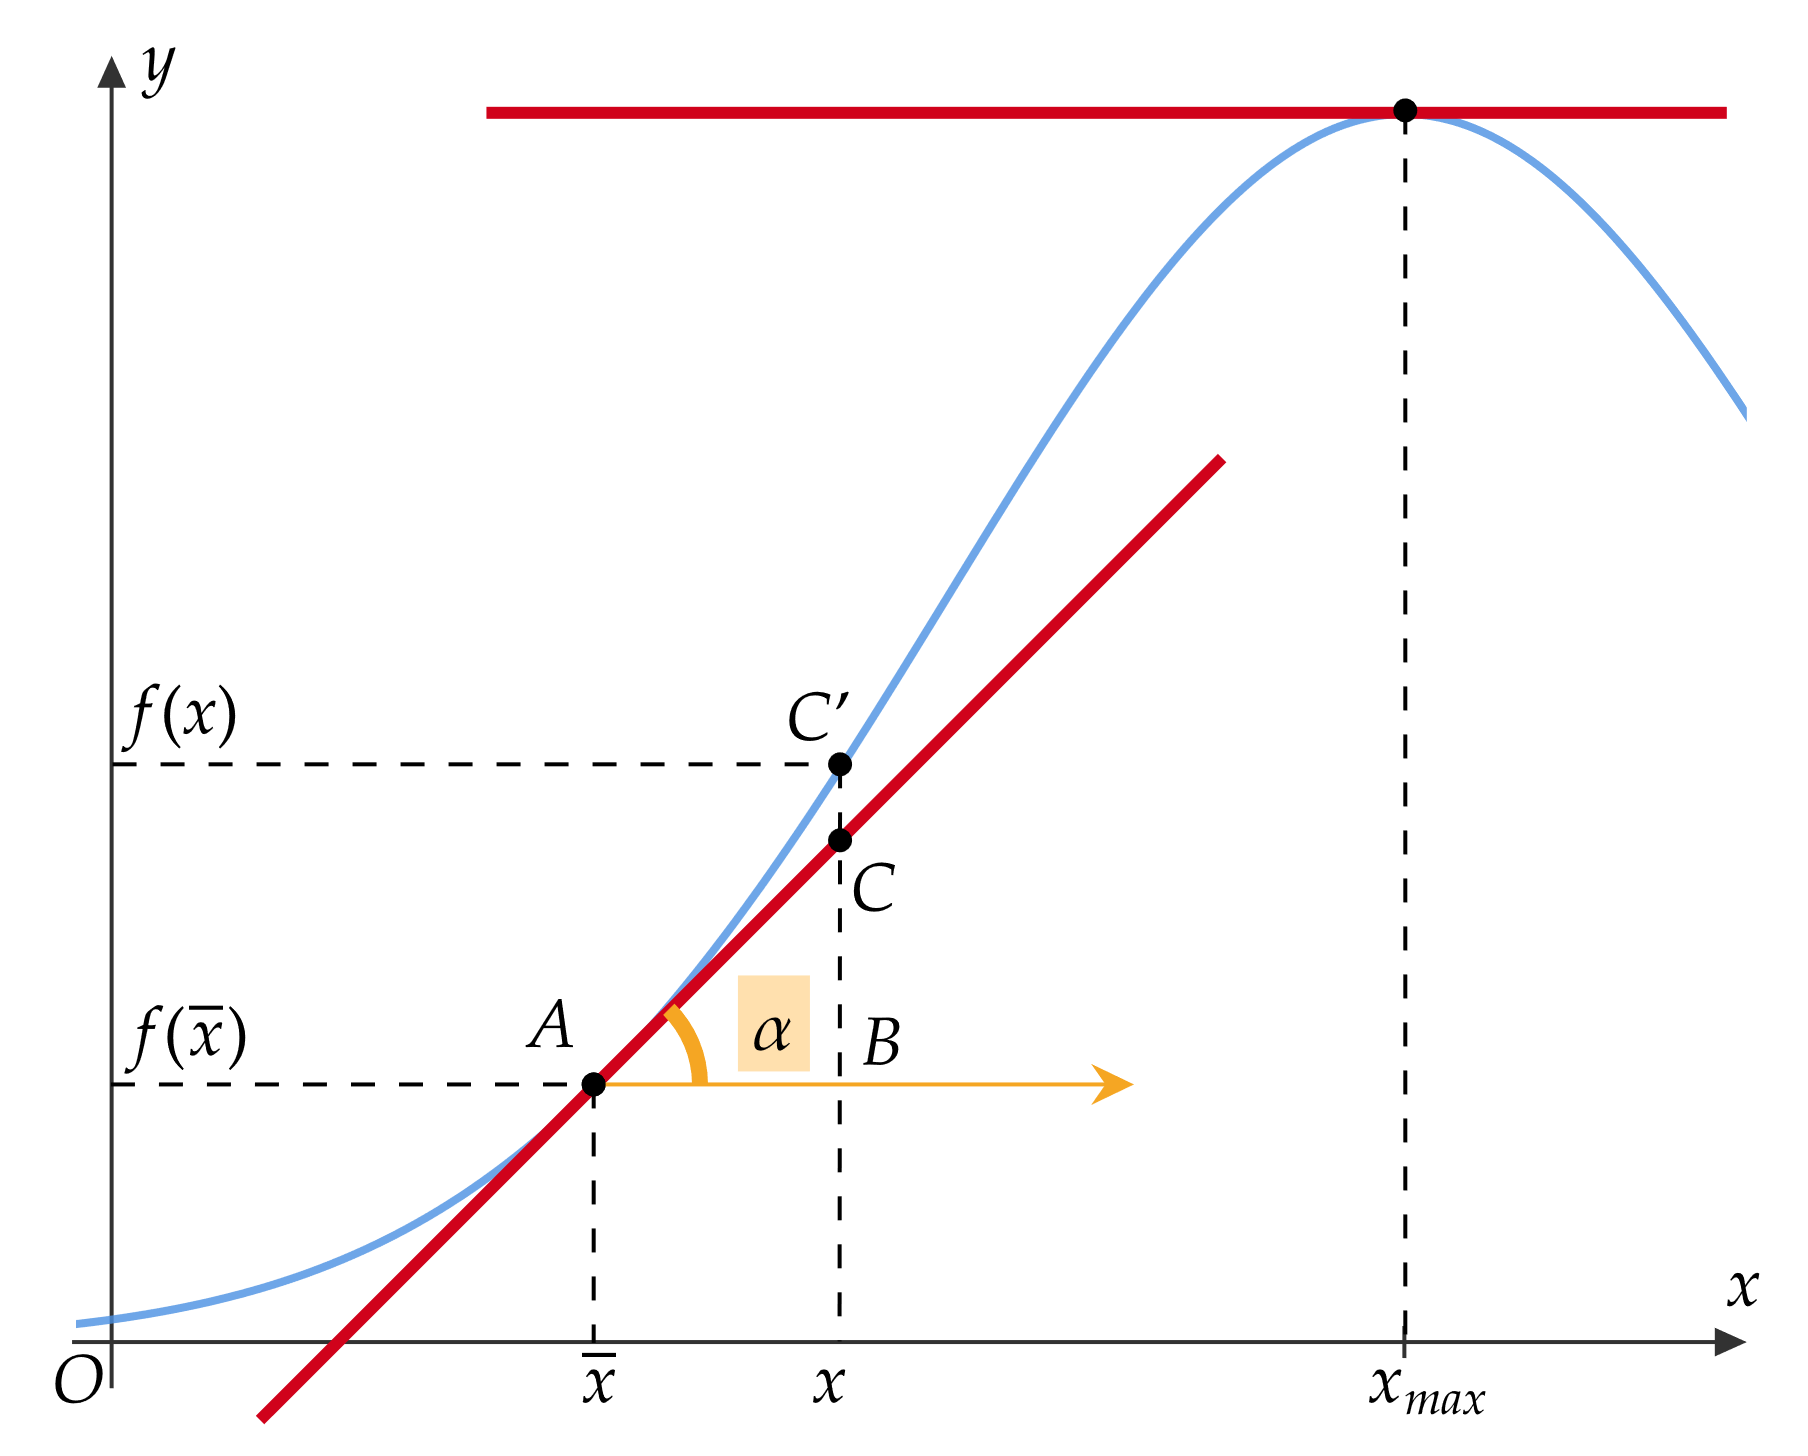
\includegraphics[width = 1\textwidth]{fig1.png}
    \caption{График функции $f\qty(x)$ отмечен голубым цветом. Касательные обозначены красным. Видно, что касательная в точке максимума $x_{max}$ параллельна оси $Ox$. Через $\alpha$ обозначен угол наклона касательной, касающейся графика функции $f(x)$ в точке $\overline{x}$.}
    \label{fig:1}
\end{figure}
\par
Задача отыскания экстремумов является ни чем иным, как задачей на отыскание точек, касательные к графику функции $f(x)$ в которых параллельны оси абсцисс (см. рис. \ref{fig:1}).
\par
Задача определения наклона кривой в заданной точке также связанна с определением наклона касательной, ведь наклон кривой в данной точке прямо и определяется как наклон касательной, проведённой в данной точке. Объясним смысл понятия \emph{наклон прямой}. Сперва введём угол наклона прямой.
\begin{definition}
Угол наклона прямой $\alpha$~\----~это угол между прямой и положительным направлением оси $Ox$.
\end{definition}
Данное определение облегчает объяснение понятия наклона прямой, которое вводится следующим образом.
\begin{definition}
Наклоном прямой называют тангенс угла наклона данной прямой $\tan{\alpha}$.
\end{definition}
Например, экстремум соответсвует касательной с наклоном равным $0$. На данном уровне описания тождественным понятию наклона графика функции $f(x)$ является \emph{производная функции $f(x)$}, строгое математическое определение которой будет дано ниже. Её частно обозначают с помощью штриха $f'\qty(x)$, и мы будем придерживаться данного обозначения. Попробуем вычислить значение производной в точке $\overline{x}$. Точное значение производной будет записываться следующим образом:
\begin{equation}
     f'\qty(\overline{x}) = \dfrac{CB}{AB},
\end{equation}
где обозначения взяты с рисунка \ref{fig:1}. Однако с точным значением производной есть проблема, заключающаяся в том, что мы не можем знать длину отрезка $CB$, так как, вообще говоря, нам неизвестно уравнение касательной. Поэтому нужно прибегнуть к приблежённому вычислению производной, воспользовавшись тем фактом, что 
\begin{equation}
    CB \approx C'B.
\end{equation}
Тогда можно записать, что приближённое значение производной будет вычислено так:
\begin{equation}\label{eq:5}
     f'\qty(\overline{x}) = \dfrac{CB}{AB} \approx \dfrac{C'B}{AB} = \dfrac{f(x) - f(\overline{x})}{ x-\overline{x}}.
\end{equation}
Ясно из геометрических соображений (см. рис. \ref{fig:1}), что при приближении точки $x$ к $\overline{x}$ ошибка в вычислении производной будет стремиться к нулю
\begin{equation}
    \dfrac{CB - C'B}{AB} \underset{x\rightarrow \overline{x}}{\longrightarrow} 0.
\end{equation}
Важно подчернкуть, что нужно иметь дело именно со стремлением. Если просто приравнять
\begin{equation}
    x = \overline{x},
\end{equation}
то в крайней левой части серии равенств (\ref{eq:5}) получится неопределённость типа $0/0$, чего нужно избегать. Поэтому нужно именно стремить точку $x$ к точке, где нам интересно найти производную:
\begin{equation}
    x\rightarrow \overline{x}.
\end{equation}
Данные качественные соображения можно обобщить введением строгого математического определения производной функции.
\begin{definition}\label{def:13}
Функция $f\qty(x)$ называется дифференцируемой в точке $\overline{x}$, если существует предел 
\begin{equation}
    \lim_{x\rightarrow \overline{x}}{\dfrac{f(x) - f(\overline{x})}{ x-\overline{x}}} = A,
\end{equation}
то есть если 
\begin{equation}
    \forall \varepsilon > 0\ \exists \delta > 0\eval \forall x \in \qty(\overline{x} - \delta, \overline{x} + \delta) \Longrightarrow \abs{\dfrac{f(x) - f(\overline{x})}{ x-\overline{x}} - A} < \varepsilon.
\end{equation}
Данный предел, если существует, называется производной функции $f\qty(x)$ в точке $\overline{x}$ и обозначается следующим образом:
\begin{equation}
    f'\qty(\overline{x}) = \dv{f}{x}\eval_{\overline{x}} = f_x \qty(\overline{x}).
\end{equation}
\end{definition}
Данное определение является частным случаем определения предела функции, что будет показано ниже.

\subsection{Значение действительного числа}
Пускай нам нужно записать значение действительного числа: например, требуется как можно более точно вычислить значение длины окружности радиуса $R$. По определению длина окружности составляет $2\pi R$. Если радиус окружности не кратен числу, обратному числу $\pi$, то длина окружности не может быть записана в рациональных числах, имеющих вид 
\begin{equation}
    \dfrac{m}{n},\ m,n \in \mathbb{Z},\ n\ne 0.
\end{equation}
Именно с рациональными числами оперируют при практических вычислениях, потому что их можно записать в виде конечной либо периодической десятичной дроби. 
\par
Как же быть с иррациоанльными числами? Их полная десятичная запись не представляется возможной, зато их можно с требуемой точностью приблизить рациональными числами. Это делается с помощью теории пределов, например, организуется некоторая последовательность рациональных чисел, сходящаяся к заданному иррациональному числу. То есть это ещё один пример использования теории пределов в математическом анализе, позволяющий с любой заданной точностью определить требуемое иррациональное число.

\subsection{Интеграл}
В физических науках часто ставится задача вычисления площади под кривой. Пускай, например, задана некоторая функциональная зависимость $f(x)$ и требуется вычислить площадь \emph{криволинейной трапеции} (см. рис. \ref{fig:2}), то есть фигуры, ограниченной осью абсцисс, функциональной кривой и двумя параллельными прямыми 
\begin{equation}
    x = a, \quad x = b.
\end{equation}
\begin{figure}
    \centering
    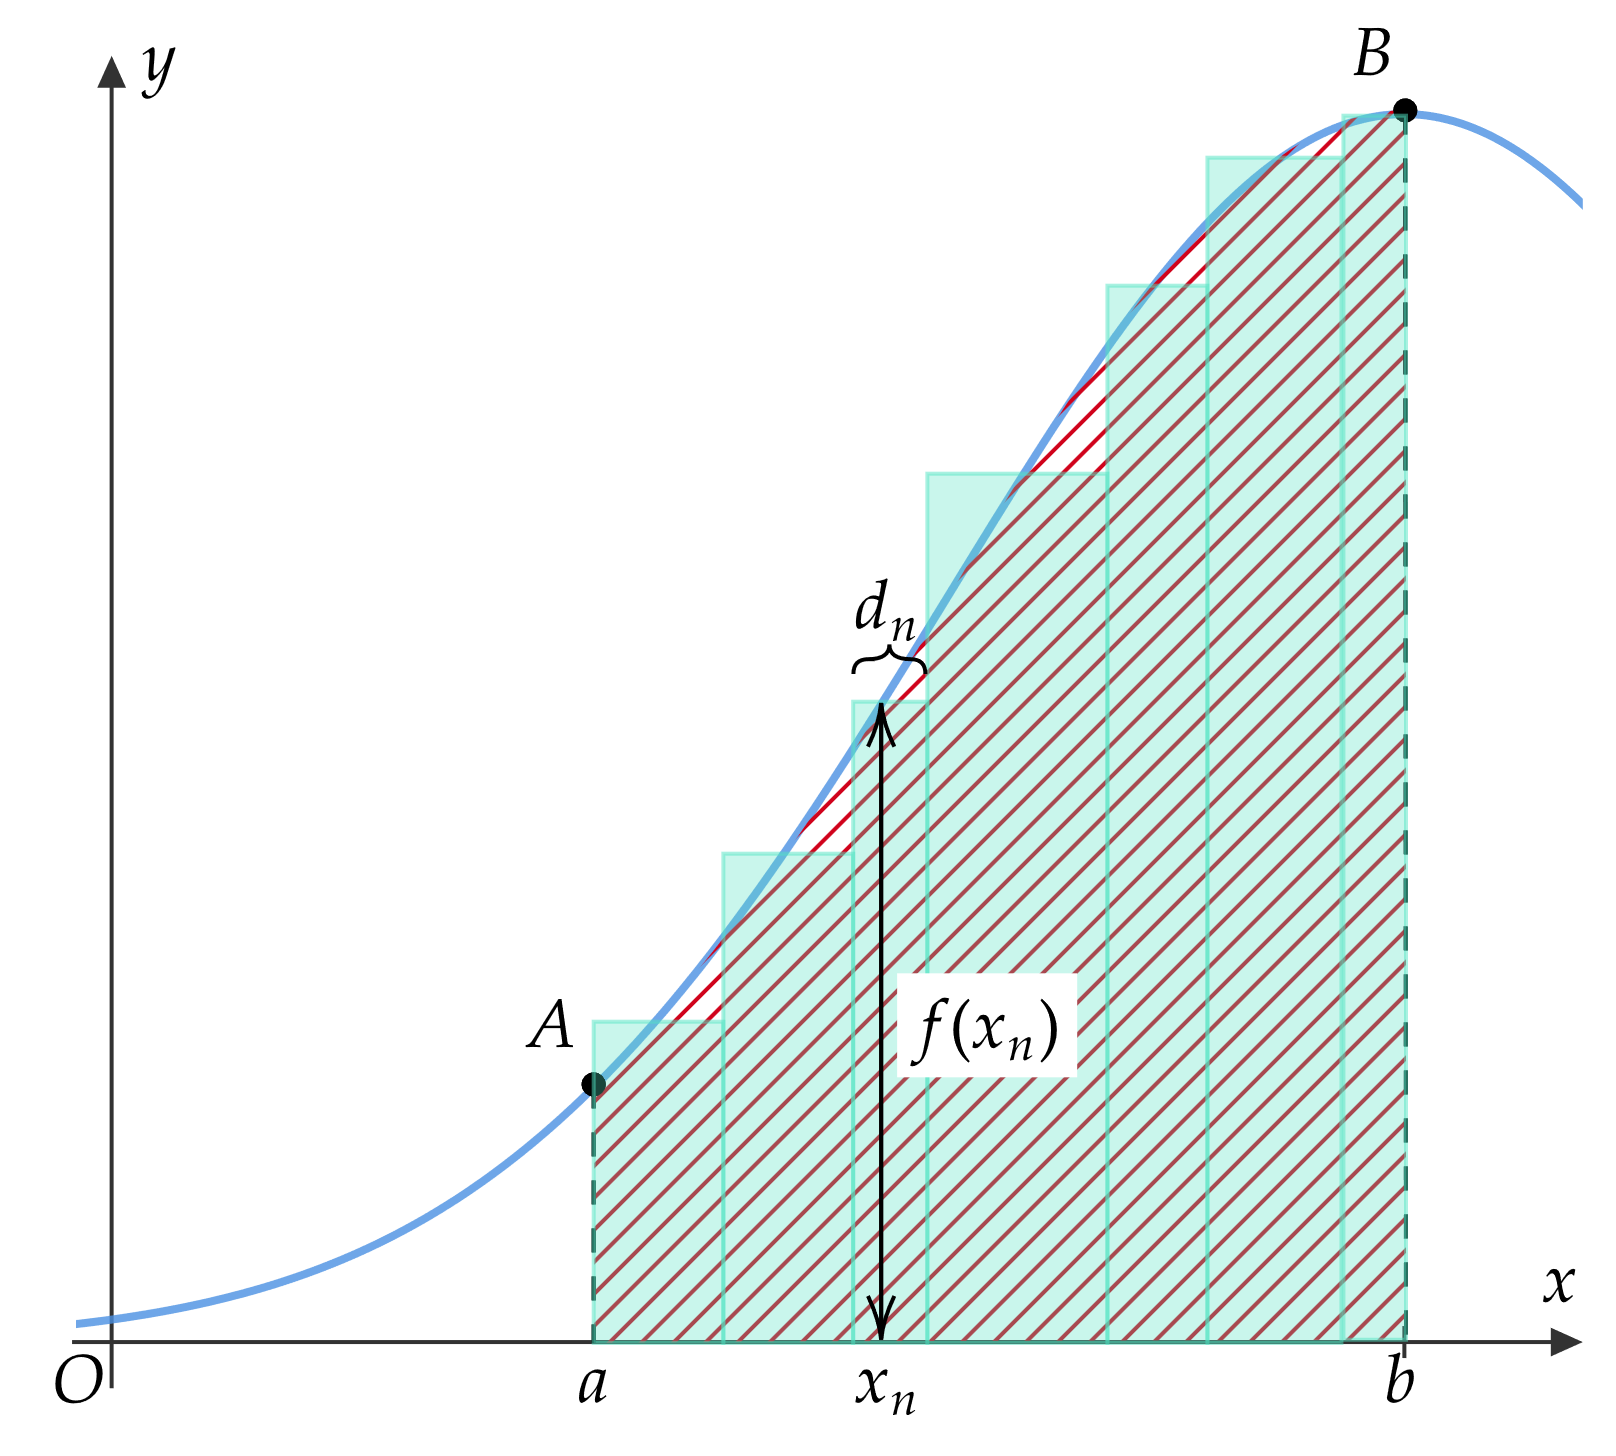
\includegraphics[width = 1\textwidth]{fig2.png}
    \caption{График функции $f\qty(x)$ отмечен голубым цветом. Область, покрытая красной штриховкой, соответсвует площади, занятой криволинейной трапецией.}
    \label{fig:2}
\end{figure}
Будем исходить из того, что мы лишь знаем, что площадь прямоугольника равна произведению его сторон. Так площадь прямоугольника со сторонами $a,\ b$ будет равна
\begin{equation}
    S = a\cdot b.
\end{equation}
Это знание совершенно никак не позволяет вычислить площадь такой сложной фигуры, какой является криволинейная трапеция. Тогда предложим приближённый способ вычисления площади криволинейной трапеции (см. рис. \ref{fig:2}). Можно разбить интервал $\qty(a,b)$ на отрезочки длины $d_n$. На каждом из таких отрезочков выбрать точку $x_n$ случайным образом. Тогда сумма площадей прямоугольников со сторонами $d_n,\ f(x_n)$ будет приближать площадь криволинейной трапеции:
\begin{equation}
    S \approx \sum_{n=0}^{N} d_n \cdot f(x_n).
\end{equation}
Можно получить приближение со сколь угодно высокой точностью с помощью всё более частого разбиения интевала $\qty(a,b)$ на отрезки длины $d_n$.
\par
Поэтому площадь криволинейной трапеции определяют через предел следующим образом:
\begin{equation}
    S = \underset{\Delta \rightarrow 0}{\lim_{N \rightarrow \infty}}\ { \sum_{n=0}^{N} d_n \cdot f(x_n)}, \quad \Delta = \max_{n\in \qty[0,N]}{d_n}.
\end{equation}
Более полно и строго данный вопрос будет рассмотрен позже. А пока остановимся на том, что под \emph{определённым интегралом от функции $f\qty(x)$ по отрезку $[a,b]$} понимают площадь криволинейной трапеции, то есть фигуры, ограниченной графиком функции $f(x)$, осью абсцисс и двумя параллельными прямыми 
\begin{equation}
    x=a,\quad x=b.
\end{equation}
Определённый интеграл обозначается следующим образом:
\begin{equation}
    \int_{a}^{b} f\qty(x) \dd x.
\end{equation}
Прошлые выводы о площади криволинейной трапеции справедливы тождественно для определённого интеграла. Так, например, верно следующее определение через предел:
\begin{equation}\label{eq:int}
    \int_{a}^{b} f\qty(x) \dd x = \underset{\Delta \rightarrow 0}{\lim_{N \rightarrow \infty}}\ { \sum_{n=0}^{N} f(x_n) \cdot d_n}, \quad \Delta = \max_{n\in \qty[0,N]}{d_n}.
\end{equation}

\section{Предел функции}
\subsection{Определение}
Перед тем, как определить предел функции, нужно сначала понять, что понимается под функцией. Определим данное понятие.
\begin{definition}
Действительнозначной функцией $\Psi$ аргумента из множества $\mathbb{X}$ называется отображение из множества $\mathbb{X}$ во множество действительных чисел. Данные слова записываются следующим образом:
\begin{equation}
    \Psi : \mathbb{X}\longrightarrow\mathbb{R}.
\end{equation}
\end{definition}
То есть функция является правилом, по которому каждому элементу из $\mathbb{X}$ ставится в соответсвие действительное число. Перед тем, как переходить к определению предела функции, нужно ввести понятие проколотой окрестности. Хотя для ряда специфичных пределов требуется доопределять понятие проколотой окрестности (об этом будет сказано ниже), но в стандартных случаях используют следующее достаточно универсальное определение.
\begin{definition}\label{def:o}
Пускай для множества $\mathbb{X}$ (на котором определена рассматриваемая функция $\Psi$) определено правило вычисления расстояния между двумя элементами, то есть задано
\begin{equation}
    \rho\qty(x,y), \quad \forall x,y \in \mathbb{X}.
\end{equation}
Тогда проколотой $\varepsilon$\--окрестностью точки $x\in \mathbb{X}$ называется множество таких точек множества $\mathbb{X}$, что расстояние между каждой из них и точкой $x$ меньше либо равно $\varepsilon$ и строго положительно. Записывается данное определение так:
\begin{equation}
    O_\varepsilon \qty(x) = \qty{y\eval y \in \mathbb{X},\ 0<\rho\qty(x,y) \le \varepsilon}.
\end{equation}
\end{definition}
Теперь перейдём к определению предела функции.
\begin{definition}\label{def:23}
Пределом функции $\Psi\qty(x)$ при стремлении $x$ к $*$ называется такое число $A \in \mathbb{R}$
\begin{equation}
    \lim_{x\rightarrow *}{\Psi\qty(x)} = A,
\end{equation}
что для него верно следующее:
\begin{equation}
    \forall \varepsilon > 0\ \exists \delta\qty(\varepsilon) > 0 \eval \forall x \in O_\delta\qty(*) \Longrightarrow \abs{\Psi\qty(x) - A} < \varepsilon.
\end{equation}
\end{definition}
\subsection{Замечание}
Определение (\ref{def:23}) описывает лишь конечные пределы, то есть оно подходит для тех случаев, когда 
\begin{equation}
    \abs{A} < +\infty.
\end{equation}
Если же в рассматриваемом случае, например,
\begin{equation}
    A = +\infty,
\end{equation}
то определение предела легко модифицируется под такое значение $A$. Нужно лишь теперь потребовать от определения, чтобы оно отражало тот факт, что значение функции $\Psi$ начинает неограниченно возрастать. То есть для сколь угодно больших $\varepsilon$ можно найти такую окрестность аргументов функции $\Psi$, что значение функции $\Psi$ будет больше $\varepsilon$. Данные слова записываются с помощью кванторов следующим образом.
\begin{definition}\label{def:24}
\begin{equation}
    \lim_{x\rightarrow *}{\Psi \qty(x)} = +\infty \Longleftrightarrow \forall \varepsilon > 0\ \exists \delta\qty(\varepsilon) > 0 \eval \forall x \in O_\delta\qty(*) \Longrightarrow \Psi\qty(x) > \varepsilon.
\end{equation}
\end{definition}

Кроме того, стоит обратить внимание, что $*$ может не лежать во множестве $\mathbb{X}$, где определена функция $\Psi$, тогда для справедливости определения (\ref{def:23}) порой требуется, чтобы для расширенного множества 
\begin{equation}
    \mathbb{Y} = \mathbb{X}\cup\qty{*}
\end{equation}
должно быть переопределено понятие окрестности. Так, например, для того, чтобы написать определение предела функции $f(x)$, определённой над множеством действительных чисел, при $x$, стремящемся к $+\infty$, нужно определить $\varepsilon$\--окрестность бесконечности следующим образом:
\begin{equation}\label{eq:o}
    O_\varepsilon\qty(+\inf) = \qty{y\eval y\in \mathbb{R}, \ y > \varepsilon}.
\end{equation}
Данная окрестность автоматически получается проколотой, так как все её члены являются действительными числами, поэтому не могут обратиться в бесконечность. Тогда определение (\ref{def:23}), где под $*$ стоит понимать $+\infty$, описывает конечный предел функции при стремлении аргумента к положительной бесконечности.
\par
Иными словами, для сколь угодно малого $\varepsilon$ найдётся такое большое $\delta$, что для любого $x>\delta$ значение функции $\Psi\qty(x)$ будет $\varepsilon$\--близко к значению предела $A$. В математических обозначениях и с использованием окрестности, определённой в (\ref{eq:o}), эти слова выражаются так:
\begin{equation}
    \lim_{x\rightarrow +\infty}{\Psi \qty(x)} = A \in \mathbb{R} \Longleftrightarrow \forall \varepsilon > 0\ \exists \delta\qty(\varepsilon) > 0 \eval \forall x \in O_\delta\qty(+\infty) \Longrightarrow \abs{\Psi\qty(x) - A} < \varepsilon.
\end{equation}


\section{Примеры использования предела в математическом анализе: завершение}
\subsection{Производная}
Определение производной (\ref{def:13}) является частным случаем определения предела функции (\ref{def:23}), где функция 
\begin{equation}
    \Psi\qty(x) = \dfrac{f(x) - f(\overline{x})}{ x-\overline{x}},
\end{equation}
определённая на множестве
\begin{equation}
    \mathbb{X} = \mathbb{R}\setminus\qty{\overline{x}},
\end{equation}
где точка $\overline{x}$ исключена, ибо в данной точке функция $\Psi\qty(x)$ обращается в неопределённость типа $0/0$. А звёздочка в определении предела функции в нашем случае положена равной $\overline{x}$. То есть мы имеем ситуацию, когда 
\begin{equation}
    *=\overline{x}\notin \mathbb{X}.
\end{equation}
Однако это по сути не важно, так как вычислить расстояние между двумя точками прямой действительных чисел мы в состоянии и работает обычное определение проколотой окрестности (\ref{def:o}).
\subsection{Предел последовательности}
Последовательность действительных чисел $\qty{a_n}_{n=0}^\infty$ является функцией натуральных чисел, что можно записать так:
\begin{equation}
    \Psi: \mathbb{N}\longrightarrow\mathbb{R}, \quad \Psi(n) = a_n,\ n \in \mathbb{N}.
\end{equation}
Тогда определение предела последовательности тоже является частным случаем определения предела функции (\ref{def:23}), где 
\begin{equation}
    \mathbb{X} = \mathbb{N},\quad *=\infty\notin \mathbb{X}.
\end{equation}
Поэтому требуется переопределить понятие окрестности следующим образом:
\begin{equation}
    O_\varepsilon\qty(\infty) = \qty{m\eval m\in \mathbb{N},\ m>\varepsilon}.
\end{equation}
Подставляя данные объекты в определение предела функции, получим определение предела последовательности, которое было изучено на предыдущей лекции \cite{lim}.

\subsection{Интеграл}
Попробуем определить определённый интеграл через предел функции (\ref{def:23}). Прежде всего нужно разобраться со множеством $\mathbb{X}$. Для этого обратимся к понятию \emph{разбиения интервала $\qty(a,b)\subset \mathbb{R}$} (см. рис. \ref{fig:3}). 
\begin{figure}
    \centering
    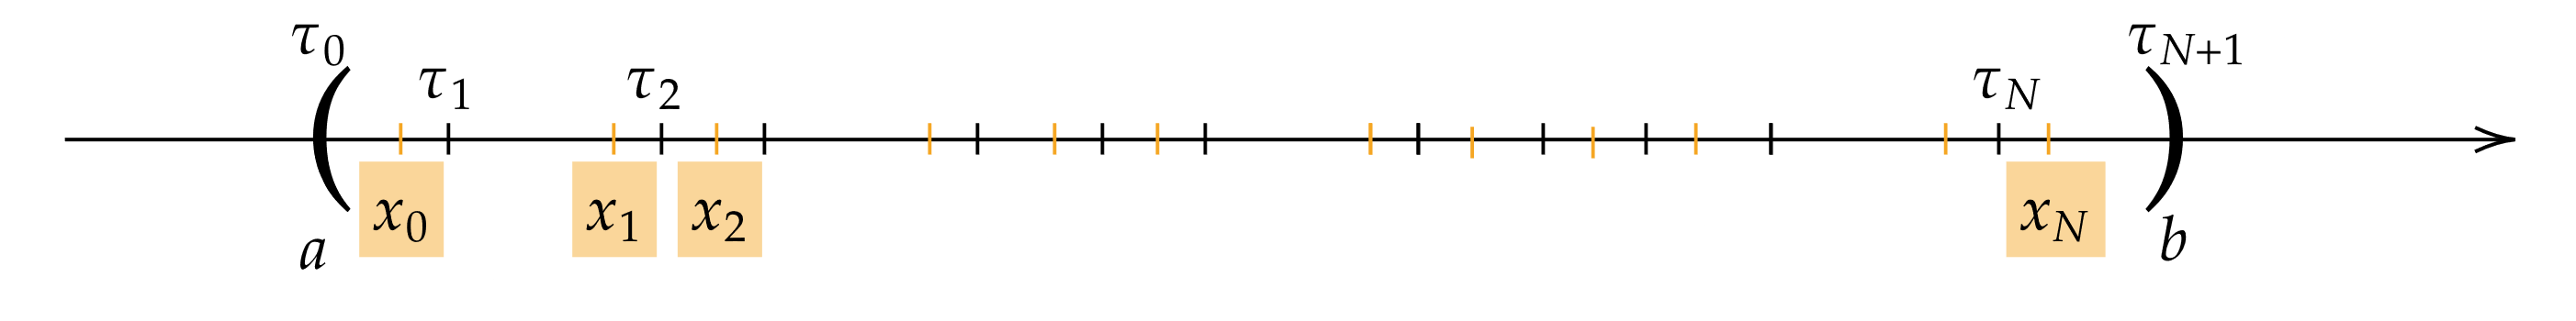
\includegraphics[width = 1\textwidth]{fig3.png}
    \caption{Иллюстрация разбиения со множеством граничных точек $\qty{\tau_n}$ и множеством точек, в которых будет вычисляться значение функции $\qty{x_n}$. }
    \label{fig:3}
\end{figure}
Под ним мы будем понимать совокупность набора граничных точек 
\begin{equation}
    \qty{\tau_n}_{n=0}^{N+1}, \quad a=\tau_0<\tau_1<\ldots<\tau_N<\tau_{N+1}=b
\end{equation}
с набором точек, в которых вычисляется значение функции:
\begin{equation}
    \qty{x_n}_{n=0}^N,\quad x_n \in \qty[\tau_n,\tau_{n+1}].
\end{equation}
Множество всех разбиений и будет множеством $\mathbb{X}$. Теперь определимся с тем, чем будет в определении определённого интеграла $*$. Как было качественно показано выше в формуле (\ref{eq:int}), при стремлении разбиения ко всё более мелкому, то есть при стремлении набора граничных точек ко всё более частому, интегральная сумма 
\begin{equation}
    \sum_{n=0}^{N} d_n \cdot f(x_n), \quad d_n = \tau_{n+1} - \tau_{n}
\end{equation}
будет всё лучше и лучше приближать площадь криволинейной трапеции, что мы и хотим получить. Поэтому звёздочкой надо положить бесконечно мелкое разбиение, то есть такое разбиение, при котором расстояние между соседними граничными точками стремится к нулю. Проколотую $\varepsilon$\--крестность тогда стоит выбрать так:
\begin{equation}
    O_\varepsilon = \qty{x\eval x\in \mathbb{X},\ 0<\max_{n\in\qty[0,N]}\qty{\tau_{n+1} - \tau_n}<\varepsilon}.
\end{equation}
Осталось подставить введённые объекты в определение предела функции и мы получим определение определённого интеграла.

\subsection{Предел и вещественные числа}
Рассмотрим единичную окружность (см. рис. \ref{fig:4}), ясно, что её длина будет равна $2\pi$, но как вычислить данное значение численно с заданной точностью?  
\begin{figure}
    \centering
    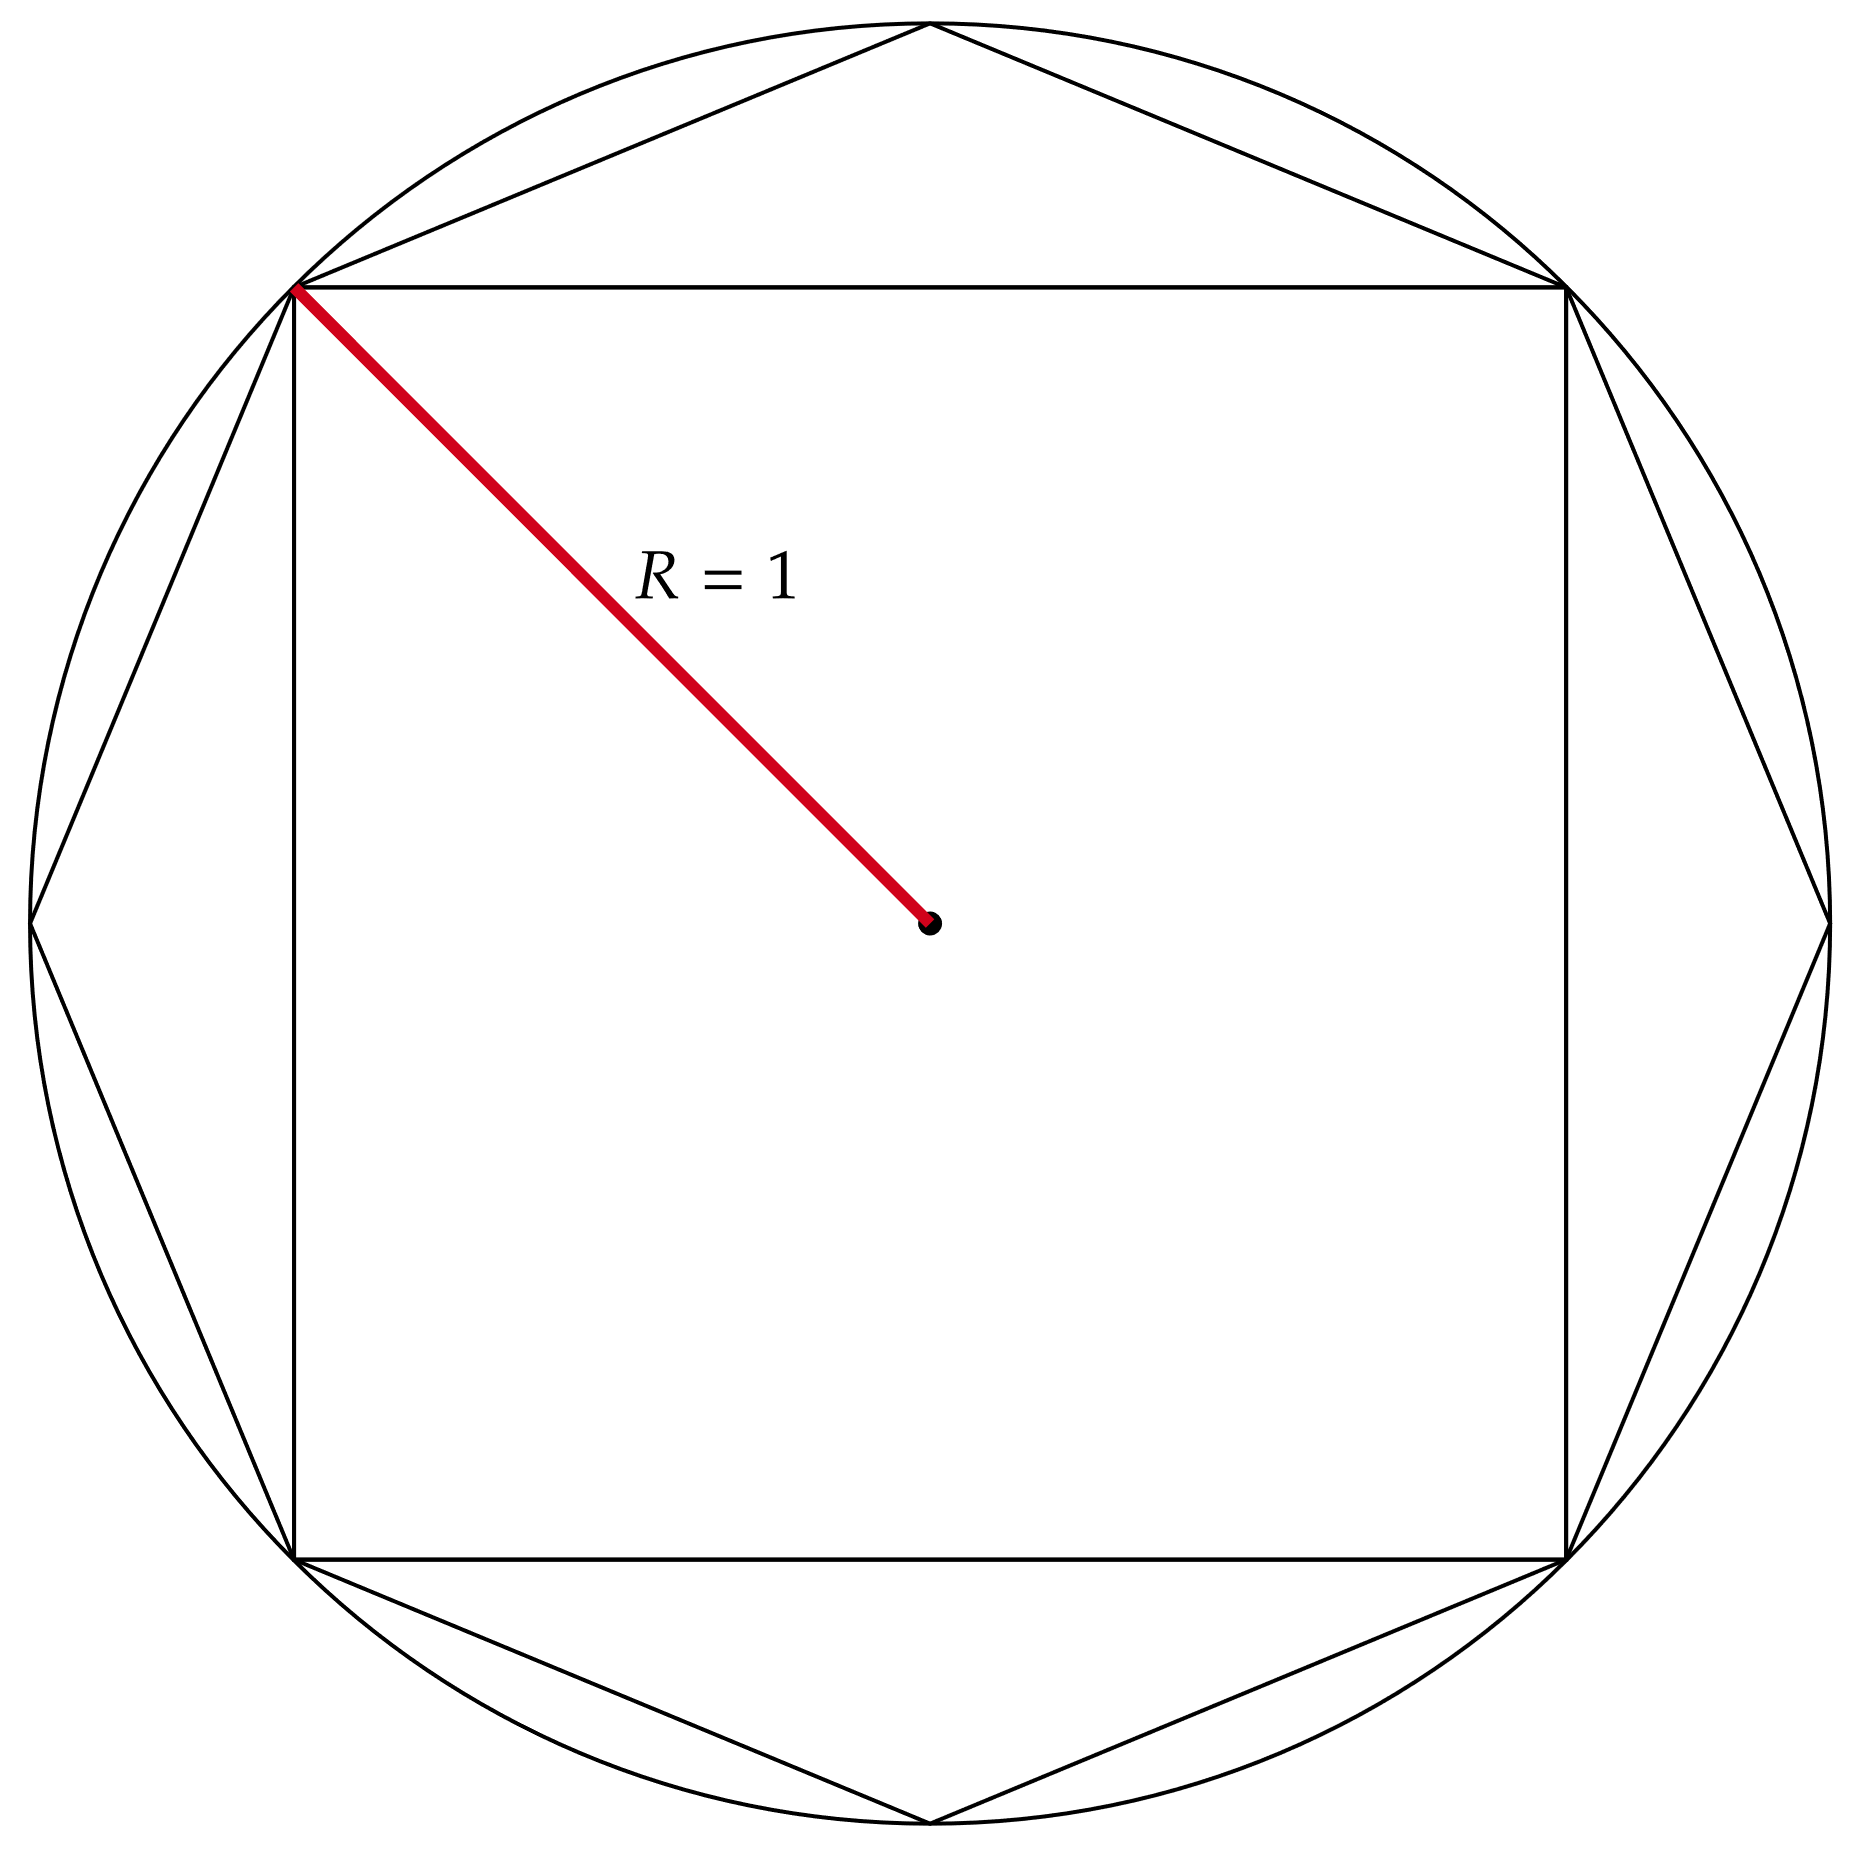
\includegraphics[width = 1\textwidth]{fig4.png}
    \caption{Иллюстрация к вычислению длины окружности c единичным радиусом. Видно, что при увеличении количества сторон правильного $n$\--угольника, периметр фигуры стремится к длине окружности.}
    \label{fig:4}
\end{figure}
\par
Можно использовать следующий геометрический метод (см. рис. \ref{fig:4}). Давайте вписывать в окружность правильные $n$\--угольники со всё большим количеством сторон. Геометрически видно, что с увеличением числа сторон периметр фигуры всё больше похож на длину окружности $2\pi$. Действительно, длина стороны правильного $n$\--угольника, вписанного в единичную окружность, равна $\sin\qty(2\pi/n)$ (должно быть ясно, так как это обычная школьная формула). Очевидно, что периметр фигуры будет тогда
\begin{equation}
    P_n = n \cdot \sin\qty(\dfrac{2\pi}{n}).
\end{equation}
Если из геометрических соображений мы уже поняли, что предел периметров сходится к числу $2\pi$, однако аналитически на данной стадии доказать это будет трудоёмко, ведь потребуется знание первого замечательного предела, что будет рассказано сильно позже в курсе. Поэтому, опираясь лишь на геометрическую аналогию, записываем следующий результат:
\begin{equation}
    \lim_{n\rightarrow\infty}{n \cdot \sin\qty(\dfrac{2\pi}{n})} = 2\pi.
\end{equation}
Итак, теперь вспомним определение предела последовательности \cite{lim}. Из него следует, что мы можем по заданной точности (то есть для любой $\varepsilon$) найти такой номер элемента последовательности (то есть $N$), что все последующие члены последовательности приближают $2\pi$ не хуже, чем с точностью $\varepsilon$. Это и есть то, что нам хотелось найти.

\section{Цепные дроби}
\subsection{Введение}
Мы говорили о том, что можно задавать иррациональные вещественные числа как предел последовательности рациональных действительных чисел. Обратимся к пратике и рассмотрим обыкновенный лист бумаги формата A4. Характерной особенностью данного формата является то, что если сложить такой лист пополам (сгиб параллелен малой стороне), то получится лист бумаги с соотношением сторон таким же, как и у исходного листа.
\par
Данный эффект может быть достигнут только для листов с соотношением сторон $1/\sqrt{2}$. То есть одна из сторон листа должна быть больше другой в $\sqrt{2}$ раз больше. Но на практике удобно, чтобы длины сторон листов выражались целым числом миллиметром. Признаны стандартом следующие размеры листов формата A4:
\begin{equation}
    210\cross297\ \qty[\text{мм}].
\end{equation}
Отношение сторон листа A4 хорошо приближает требуемое соотношение, действительно
\begin{equation}
    \dfrac{297}{210} = 1,41428571429 \approx \sqrt{2} = 1,41421356237.
\end{equation}
\subsection{Приближение иррациональных чисел рациональными}\label{ss:42}
Иррациональные числа можно приближать рациональными различными способами. Например, можно приблизить число $\sqrt{2}$ так:
\begin{equation}
    a_0 = \dfrac{p_0}{q_0} = \dfrac{1}{1},\ a_1 =\dfrac{p_1}{q_1} = \dfrac{14}{10},\ a_2 = \dfrac{p_2}{q_2} =\dfrac{141}{100},\ \ldots
\end{equation}
Но как быстро сходится такая последовательность к $\sqrt{2}$, то есть какого качество приближения (насколько большой номер элемента последовательности нужно взять, чтобы получить приближение с заданной точностью)? Оценим для ответа на данный вопрос качество приближения $k$\--ым элементом последовательности:
\begin{equation}
    \abs{a_k - \sqrt{2}} \le \dfrac{1}{q_k}.
\end{equation}
Действительно, $k$\--ый элемент последовательности является "срезом"{} числа $\sqrt{2}$ до $k$\--ой цифры после запятой в десяточной записи, поэтому отклонение $a_k$ от $\sqrt{2}$ не может превыжать $10^{-k}$.
\subsection{Понятие о цепных дробях}
Оказывается, что можно организовать более быстросходящуюся последовательность. Метод, который позволяет это сделать, называется \emph{методом цепных дробей}. Для начала определим само понятие цепной дроби.
\begin{definition}\label{def:41}
Цепной дробью называется дробь вида
\begin{equation}
    x_n = a_0 + \dfrac{1}{a_1 + \dfrac{1}{a_2+ \dfrac{1}{a_3 + \cdots_{+\dfrac{1}{a_{n-1} + \dfrac{1}{a_n}}}}}},
\end{equation}
где $a_0$ является целым, а остальные числа $a_k$ при $k=\overline{1,n}$ являются целыми положительными.
\end{definition}

$n$\--ая цепная дробь полностью определяется $n+1$ числом $\qty{a_k}_{k=0}^n$. Если доказать, что последовательных цепных дробей сходится, то можно рассматривать бесконечную цепную дробь как предел последовательности цепных дробей.
\par
Полагая, что рассматриваемая цепная дробь сходится, покажем, как восстановливать цепную дробь для действительного числа на примере цепной дроби для $\sqrt{2}$. Для этого введём понятие \emph{остатка цепной дроби $r_n$}. Под ним будем понимать то, что осталось от бесконечной цепной дроби при "вычёркивании"{} цепной дроби $x_n$, то есть
\begin{equation}
    r_n =\dfrac{1}{a_{n+1} + \dfrac{1}{a_{n+2} + \cdots}}.
\end{equation}
Возвращаемся к примеру. Полагаем, что бесконечная цепная дробь равна $\sqrt{2}$
\begin{equation}
    x^* = \sqrt{2}.
\end{equation}
Тогда нулевой остаток цепной дроби будет записываться следующим образом:
\begin{equation}
    r_0 = x^* - a_0.
\end{equation}
$r_0$ предстваляет из себя единицу, делённую на сумму целого положительного числа и вещественного положительного числа, поэтому $r_0$ меньше единицы. Тогда $a_0$ должно быть целой частью $\sqrt{2}$
\begin{equation}
    a_0 = \qty[\sqrt{2}] = 1.
\end{equation}
Из определения остатка цепной дроби следует равенство
\begin{equation}
    r_0 = \dfrac{1}{a_1 + r_1}.
\end{equation}
Отсюда находим $r_1$ следующим образом:
\begin{equation}
    r_1 = \dfrac{1}{r_0} - a_1  = \dfrac{1}{\sqrt{2} - 1} -  a_1 = \sqrt{2} + 1 - a_1.
\end{equation}
Число $r_1$ опять же должно быть меньше единицы и больше нуля, так как оно представляет из себя единицу, делённую на сумму целого положительного числа и вещественного положительного числа. Отсюда имеем
\begin{equation}
    a_1 = \qty[\sqrt{2}+1] = 2, \quad r_1 = \sqrt{2} - 1.
\end{equation}
Замечаем, что остаток равен предыдущему
\begin{equation}
    r_0 = r_1 = \sqrt{2} - 1.
\end{equation}
Это означает, что процесс зациклился. Действительно, чтобы получить $r_2$, нужно подставить $r_1$ в формулу, в точности аналогичную формуле для $r_1$:
\begin{equation}
    r_2 = \dfrac{1}{r_1} - a_2.
\end{equation}
Если подставить сюда $r_1 = \sqrt{2} - 1$, то получим для $a_2$ тот же результат, что был получен для $a_1$. Таким образом, мы получили следующее:
\begin{equation}
    a_1 = a_2 = \ldots = 2.
\end{equation}
Таким образом, мы получаем бесконечную цепную дробь для числа $\sqrt{2}$
\begin{equation}
    \sqrt{2} = 1 + \dfrac{1}{2+\dfrac{1}{2+\dfrac{1}{2+\cdots}}}.
\end{equation}
\par
Разберёмся, как устроена последовательность цепных дробей. Сначала отметим $x_0 = a_0$ (см. рис. \ref{fig:5}). Далее замечаем, что $x_1$ больше $x_0$, так как $x_1 = a_0 + 1/a_1$. Поэтому $x_1$ будет лежать правее нулевого члена последовательности. Далее мы должны отметить $x_2 = a_0 + 1/(a_1+ 1/a_2)$, так как знаманатель второго слагаемого увеличился по сравнению с $x_1$, то число $x_2$ будет меньше $x_1$. И так далее. Видно, что последовательность имеет чередующееся направление роста и сходится к $x^*$.
\begin{figure}
    \centering
    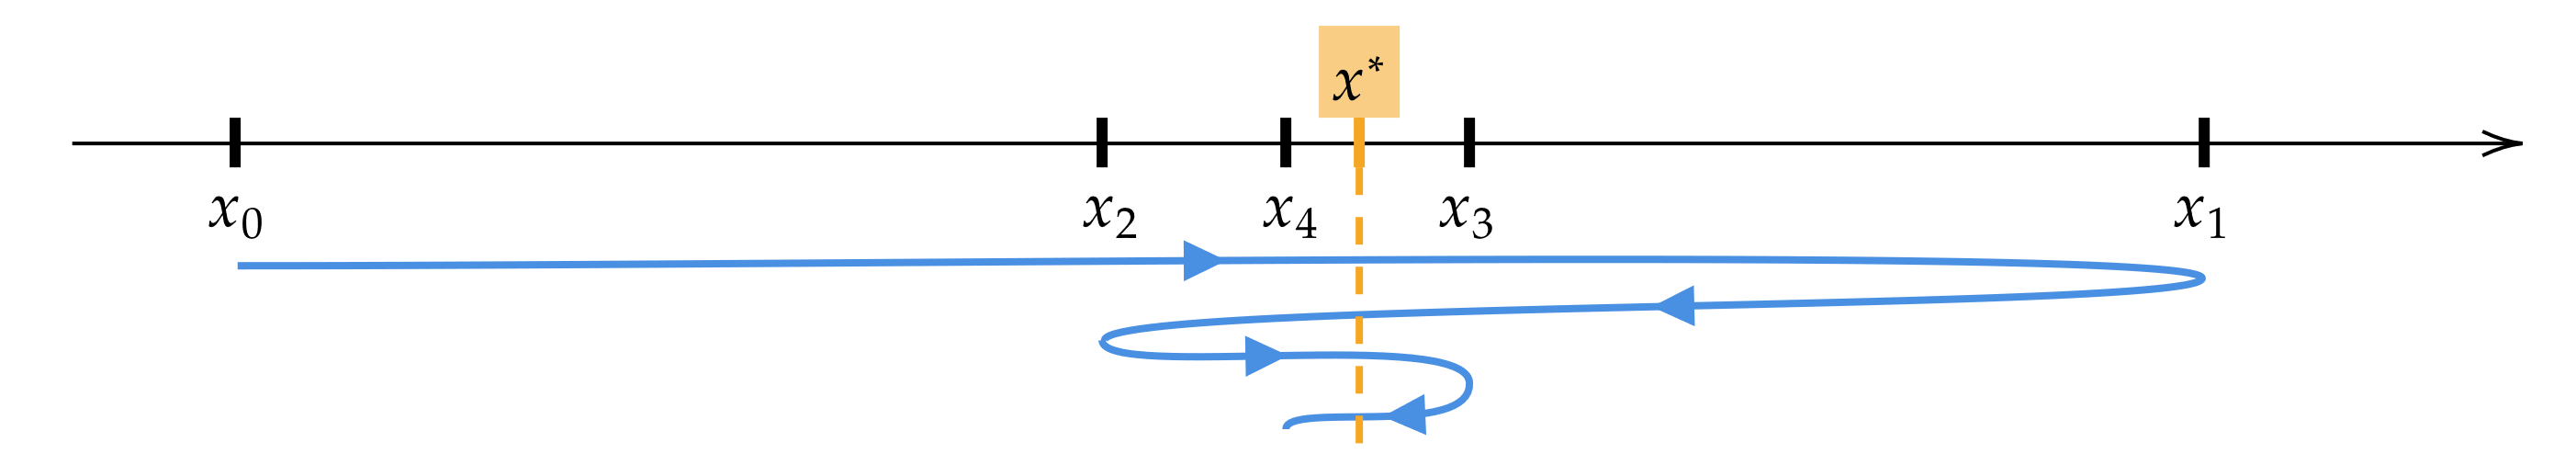
\includegraphics[width = 1\textwidth]{fig5.png}
    \caption{Изображение последовательности цепных дробей. Видно, что последовательность имеет чередующееся направление роста и сходится к $x^*$.}
    \label{fig:5}
\end{figure}
\par
Попробуем записать цепную дробь в виде обычной дроби
\begin{equation}
    x_n = \dfrac{p_n}{q_n}.
\end{equation}
Ясно, что для $x_0$ числитель и знаменатель будут иметь такой вид:
\begin{equation}\label{eq:58}
    p_0 = a_0,\quad q_0 = 1.
\end{equation}
Для первого члена получим следующий результат:
\begin{equation}\label{eq:59}
    p_1 = a_0 a_1 + 1,\quad q_1 = a_1.
\end{equation}
Можно продолжать и дальше, но попытаемся записать $x_n$ как функцию от $a_n$. Это будет дробно\--линейная функция
\begin{equation}\label{eq:60}
    x_n\qty(a_n) = \dfrac{\alpha a_n + \beta}{\gamma a_n + \delta},
\end{equation}
где греческие буквы обозначают какие\--то константы. Действительно, для $x_1$ и $x_0$ данный вид зависимости справедлив. Для остальных же цепных дробей можно доказать по методу математической индукции верность формулы (\ref{eq:60}), что читатель может сделать, опираясь на знания, полученные в школьном курсе математики.
\par
Исследуем поведение дробно\--линейной функции (\ref{eq:60}) при стремлении $a_n$ к $+\infty$ и при стремлении к $0$. Во\--первых, при стремлении к $0$ получаем следующий очевидный результат:
\begin{equation}
    \lim_{a_n \rightarrow 0}{x_n\qty(a_n)} = \dfrac{\beta}{\delta}.
\end{equation}
Посмотрим на это с другой строны. Обратимся к записи цепной дроби $x_n$ по определению \ref{def:41}:
\begin{equation}
    x_n = a_0 + \dfrac{1}{a_1 + \dfrac{1}{a_2+ \dfrac{1}{a_3 + \cdots_{+\dfrac{1}{a_{n-2} +\dfrac{1}{a_{n-1} + \dfrac{1}{a_n}}}}}}}.
\end{equation}
Тут при стремлении $a_n$ к $0$ получается, что 
\begin{equation}
    \dfrac{1}{a_{n-1}+\dfrac{1}{a_n}}\underset{a_n\rightarrow0}{\longrightarrow}0.
\end{equation}
Значит, цепная дробь $x_n$ при стремлении $a_n$ к $0$ стремится к $x_{n-2}$
\begin{equation}
    x_n \underset{a_n\rightarrow0}{\longrightarrow} x_{n-2} = \dfrac{p_{n-2}}{q_{n-2}}.
\end{equation}
То есть имеет место следующее равенство:
\begin{equation}\label{eq:65}
    \dfrac{\beta}{\delta} = \dfrac{p_{n-2}}{q_{n-2}}.
\end{equation}
\par
Рассмотрим случай стремления к $+\infty$. В данном случае для вида цепной дроби как дробно\--линейной функции (\ref{eq:60}) получаем такой результат:
\begin{equation}
    \lim_{a_n \rightarrow +\infty}{x_n\qty(a_n)} = \dfrac{\alpha}{\gamma}.
\end{equation}
С другой строны для цепной дроби, записанной в том виде, который был использован в определении \ref{def:41}, следует, что
\begin{equation}
    x_n \underset{a_n\rightarrow +\infty}{\longrightarrow} x_{n-1} = \dfrac{p_{n-1}}{q_{n-1}},
\end{equation}
так как имеет место следующее очевидное равенство:
\begin{equation}
    \dfrac{1}{a_n}\underset{a_n\rightarrow +\infty}{\longrightarrow} 0.
\end{equation}
Отсюда получаем такую запись:
\begin{equation}\label{eq:69}
    \dfrac{\alpha}{\gamma} = \dfrac{p_{n-1}}{q_{n-1}}.
\end{equation}
Теперь мы владеем двумя записями (\ref{eq:65}, \ref{eq:69}), которых хватает, чтобы вывести следующие рекурентные соотношения:
\begin{equation}\label{eq:70}
    \begin{split}
        &p_n = a_n p_{n-1} + p_{n-2};\\
        &q_n = a_n q_{n-1} + q_{n-2}.
    \end{split}
\end{equation}
\subsection{Использование цепных дробей для приближения иррациональных чисел}
Выясним скорость сходимости данного метода, для этого оценим расстояние между $x_n$ и пределом последовательности цепных дробей $x^*$
\begin{equation}
    \abs{x_{n-1} - x^*} \le \abs{x_n - x_{n-1}}.
\end{equation}
Действительно, данная оценка следует из того, что последовательность цепных дробей имеет переменное направление роста (см. рис. \ref{fig:5}). Теперь поработаем с последним выражением, используя при этом рекурентные соотношения (\ref{eq:70}):
\begin{equation}
    \begin{split}
        \abs{x_n - x_{n-1}} &= \abs{\dfrac{p_n}{q_n}-\dfrac{p_{n-1}}{q_{n-1}}} = \dfrac{\abs{p_n q_{n-1} - p_{n-1} q_n}}{q_n q_{n-1}}\\
        &= \dfrac{\abs{\qty(\cancel{a_n p_{n-1}} + p_{n-2})q_{n-1}-p_{n-1}\qty(\cancel{a_n q_{n-1}} + q_{n-2})}}{q_n q_{n-1}}\\
        &=\dfrac{\abs{p_{n-1} q_{n-2} - p_{n-2} q_{n-1}}}{q_n q_{n-1}}.
    \end{split}
\end{equation}
Таким образом, мы выразили знаменатель через тоже самое выражение, но с индексами, меньшими на единицу. Ничего не мешает уменьшать индексы в знаменатиле до тех пор, пока не получим индекса, равного $0$. То есть мы пришли к такому равенству:
\begin{equation}
    \abs{x_n - x_{n-1}} = \dfrac{\abs{p_1 q_{0} - p_{0} q_1}}{q_n q_{n-1}}.
\end{equation}
Последнее выражение мы можем упростить, взяв во внимание соотношения (\ref{eq:58}, \ref{eq:59}). Тогда мы получаем
\begin{equation}
    \abs{x_n - x_{n-1}} = \dfrac{\abs{p_1 q_{0} - p_{0} q_1}}{q_n q_{n-1}} = \dfrac{\cancel{a_0 a_1}+ 1 - \cancel{a_0 a_1}}{q_n q_{n-1}} = \dfrac{1}{q_n q_{n-1}}.
\end{equation}
То есть мы оценили скорость сходимости последовательности цепных дробей следующим образом:
\begin{equation}
    \abs{x_{n-1} - x^*} \le \dfrac{1}{q_n q_{n-1}}.
\end{equation}
Можно упростить данную оценку
\begin{equation}
    \abs{x_{n-1} - x^*} \le \dfrac{1}{q_n q_{n-1}} < \dfrac{1}{q_{n-1}^2}.
\end{equation}
Таким образом, способ, основанный на цепных дробях, оказывается быстрее способа, описанного выше в подразделе \ref{ss:42}. Так, например, для числа $\sqrt{2}$ организуется следующая последовательность цепных дробей\footnote{читатель может лично проверить правильность выписанных ниже значений элементов последовательности цепных дробей}:
\begin{equation}
    1,\ \dfrac{3}{2},\ \dfrac{7}{5},\ \dfrac{17}{12},\ \dfrac{41}{29},\ \dfrac{99}{70},\ \ldots
\end{equation}
Именно отсюда и берётся используемый во всём мире стандарт для сторон листа A4
\begin{equation}
    x_5 = \dfrac{99}{70} = \dfrac{297}{210}.
\end{equation}
Пятый член последовательности цепных дробей, сходящихся к $\sqrt{2}$, приближает $\sqrt{2}$ с хорошей точностью
\begin{equation}
    \abs{x_5 - \sqrt{2}} \le \dfrac{1}{169^2} = \dfrac{1}{28\ 561}.
\end{equation}
\section{Правило Лопиталя}

Рассмотрим ещё один из способов вычисления пределов функций. Описанный ниже способ является достаточно мощным средством при взятии пределов, однако данная методика имеет ряд жёстких ограничений, о которых стоит помнить.
\subsection{Формулировка и идея доказательства}
Итак, предположим, что требуется вычислить предел следуещего вида:
\begin{equation}\label{eq:79}
    \lim_{x\rightarrow a}{\dfrac{f\qty(x)}{g\qty(x)}},
\end{equation}
где функции $f$ и $g$ становятся бесконечно малыми (либо же стремятся одновременно к $\pm \infty$) при стремлении аргумента к $a$, то есть
\begin{equation}
    \lim_{x\rightarrow a}{f\qty(x)} = \lim_{x\rightarrow a}{g\qty(x)} = 0\ (\pm\infty).
\end{equation}
Тогда ответ на вопрос о существовании предела (\ref{eq:79}), может быть дан, если существует такой предел:
\begin{equation}\label{eq:81}
    \lim_{x\rightarrow a}{\dfrac{f'\qty(x)}{g'\qty(x)}},
\end{equation}
где штрихами обозначены производные. А когда существует предел (\ref{eq:81})? Для того, чтобы данный предел вообще мог существовать необходимо наложить определённые ограничения на функции $f$ и $g$, а именно:
\begin{align}
    &\exists O\qty(a) \eval \forall x \in O\qty(a)\ \exists f'(x),\ g'(x);\\
    & g'\qty(a)\ne 0.
\end{align}
Здесь за $O\qty(a)$ обозначена некоторая проколотая окрестность точки $a$. Действительно, данные требования просто обозначают возможность существования дроби
\begin{equation}
    \dfrac{f'\qty(x)}{g'\qty(x)},
\end{equation}
ведь они постулируют дифференцируемость функций $f$ и $g$, а также отличие знаменателя от $0$.
\par
Более того, оказывается, что в данном случае, если предел (\ref{eq:81}) существует, то искомый предел равен пределу отношений производных
\begin{equation}
    \lim_{x\rightarrow a}{\dfrac{f\qty(x)}{g\qty(x)}} = \lim_{x\rightarrow a}{\dfrac{f'\qty(x)}{g'\qty(x)}}.
\end{equation}
Сформулируем строго математически данную теорему.
\begin{theorem}[Правило Лопиталя]
Если функции $f(x)$ и $g(x)$~\----~действительнозначные функции, дифференцируемые в некоторой проколотой окрестности числа $a$, где 
\begin{equation}
    a \in \qty{\mathbb{R}\cup +\infty \cup -\infty},
\end{equation}
причём справедливо следующее:
\begin{align}
    &\lim_{x\rightarrow a}{f\qty(x)} = \lim_{x\rightarrow a}{g\qty(x)} = 0\ (\pm \infty);\\
    &g'\qty(a)\ne 0;\\
    &\exists \lim_{x\rightarrow a}{\dfrac{f'\qty(x)}{g'\qty(x)}};
\end{align}
тогда существует предел
\begin{equation}
    \lim_{x\rightarrow a}{\dfrac{f\qty(x)}{g\qty(x)}} = \lim_{x\rightarrow a}{\dfrac{f'\qty(x)}{g'\qty(x)}}.
\end{equation}
\end{theorem}
\begin{proof}
Приведём идею доказательства правила Лопиталя. Рассмотрим для краткости только случай, когда 
\begin{equation}
    \lim_{x\rightarrow a}{f\qty(x)} = \lim_{x\rightarrow a}{g\qty(x)} = 0.
\end{equation}
Зададим параметрически заданную кривую (см. рис. \ref{fig:6})
\begin{equation}
    \qty{x = g\qty(\xi),\ y = f\qty(\xi)},\quad \xi\in \qty{O\qty(a)\cup a}.
\end{equation}
Так как выполняется условие
\begin{equation}
    \lim_{x\rightarrow a}{f\qty(x)} = \lim_{x\rightarrow a}{g\qty(x)} = 0,
\end{equation}
то параметрически заданный график стремится к точке $\qty{0,\ 0}$. Назовём её точкой $O$ и соеденим отрезком с некоторой точкой 
\begin{equation}
    A = \qty{g\qty(\xi),\ f\qty(\xi)}.
\end{equation}
Заметим, что, приближая $\xi$ к $a$, мы приближаем и точку $A$ к точке $O$ (из\--за непрерывности функций $f$ и $g$, что следует из их дифференцируемости \cite{il-poz}).
\begin{figure}
    \centering
    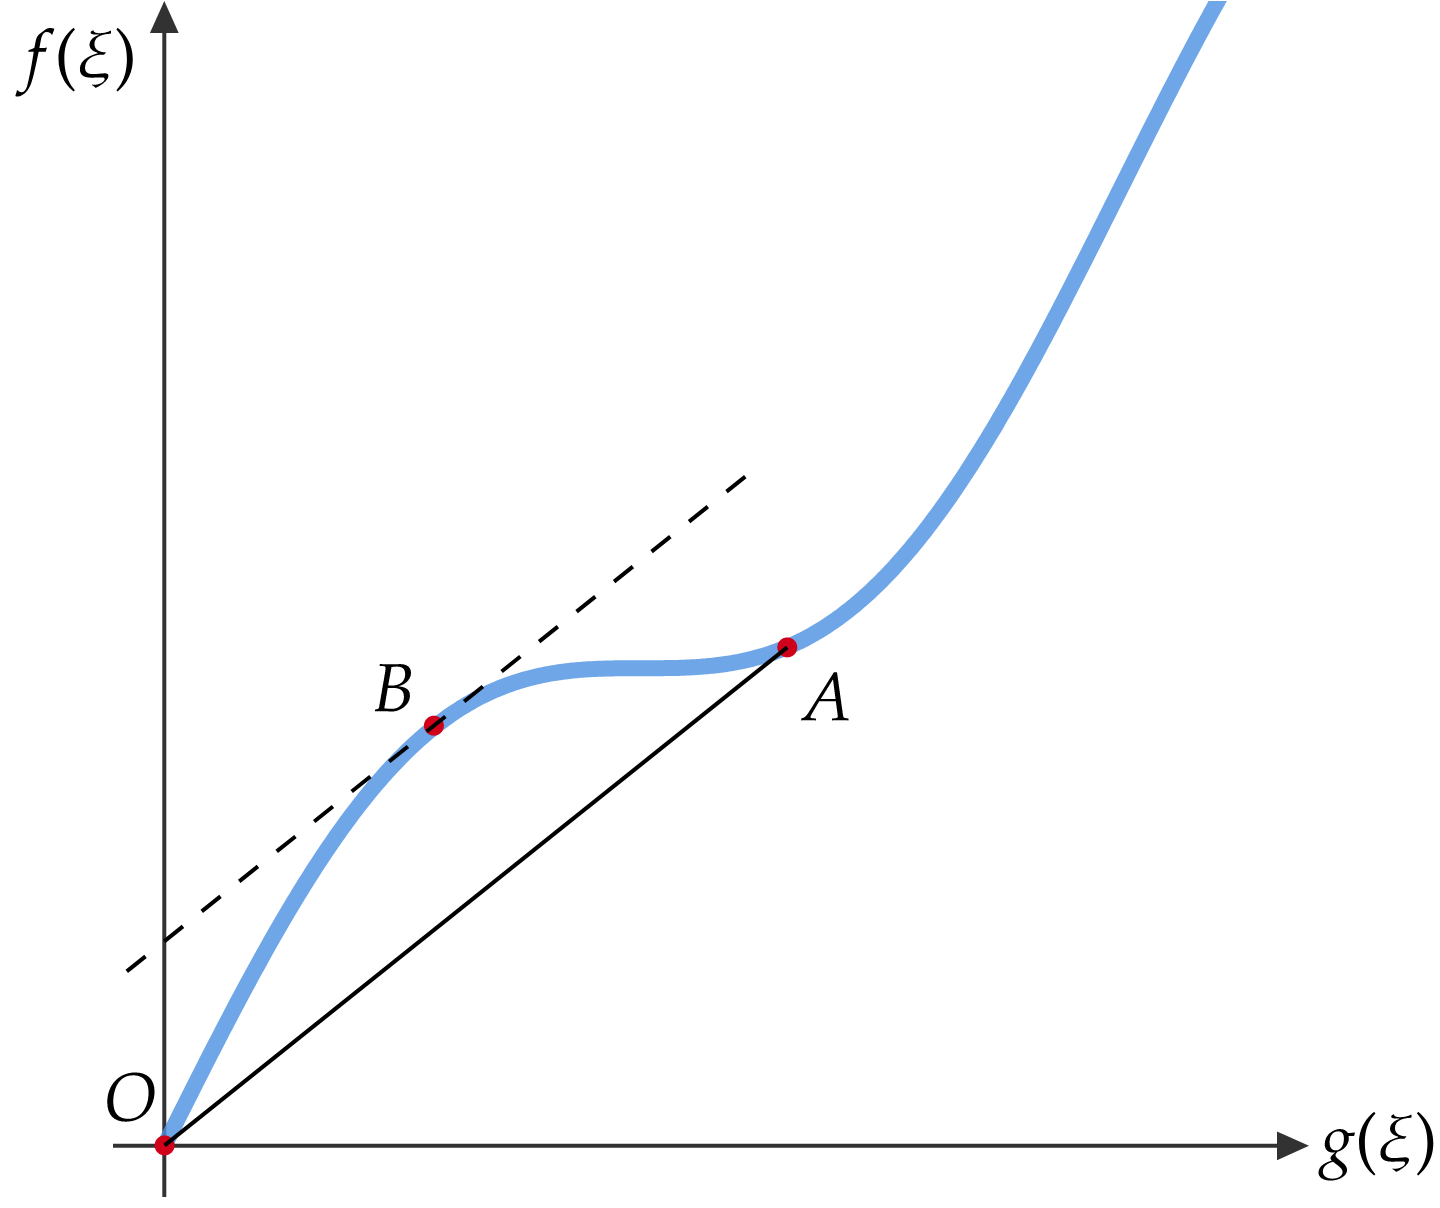
\includegraphics[width = 1\textwidth]{fig6.png}
    \caption{График параметрически заданной функции. Видно, что касательная к графику в точке $B$ параллельна хорде $OA$.}
    \label{fig:6}
\end{figure}
\par
Теперь необходимо будет прибегнуть к так называемой теореме Лагранжа \cite{il-poz}. Из данной теоремы следует, что для всякой хорды (то есть отрезка, соединяющего две точки графика функции и не имеющего более пересечений с графиком) существует точка графика функции $B$, лежащая на отрезке кривой, ограниченном хордой, что касательная параллельна данной хорде (все функции для этого должны быть непрерывны) (см. рис. \ref{fig:6}). 
\par
Теперь стремим $\xi$ к $a$, откуда следует стремление точки $A$ к точке $O$. А по теореме Лагранжа получаем, что всегда для хорды $OA$ будет находиться и касательная, проведённая к точке графика, лежащей на кусочке графика, ограниченном хордой. Как видно из рисунка $\ref{fig:7}$ при стремлении $A$ к $O$ точки $A$ и $B$ когда\--то станут неразличимы.
\begin{figure}
    \centering
    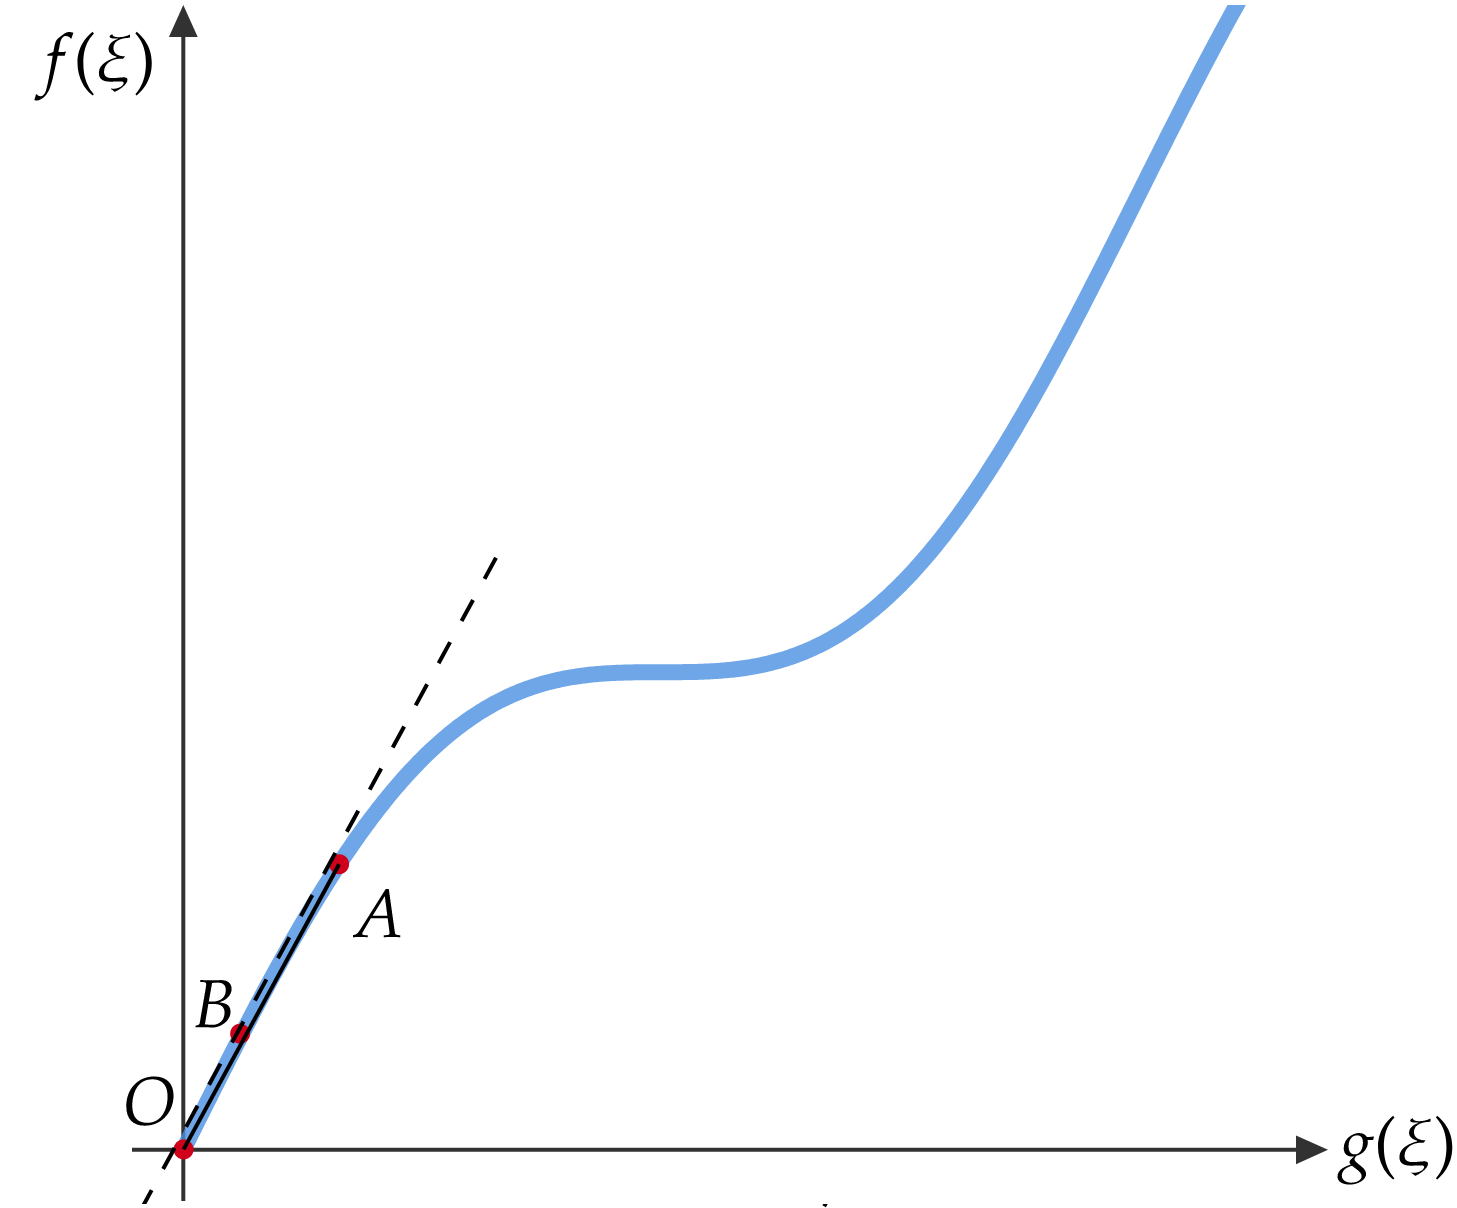
\includegraphics[width = 1\textwidth]{fig7.png}
    \caption{Рисунок, аналогичный рисунку \ref{fig:6}, только точка $A$ ближе к точке $O$. Видно, что касательная к графику в точке $B$ параллельна хорде $OA$.}
    \label{fig:7}
\end{figure}
Это значит, угол между касательной и положительным направлением оси абсцисс стремится к углу между хордой и положительным направлением оси абсцисс. Если данные углы стремятся друг к другу, то и их тангенсы тоже.
\par
Тангенс угла наклона касательной является производной функции. А производная функции, заданной параметрически, равна следующему выражению \cite{il-poz}:
\begin{equation}
    \dfrac{f'\qty(x)}{g'\qty(x)}.
\end{equation}
Так как тангенсы стремятся друг в другу, то получаем утверждение теоремы
\begin{equation}
    \lim_{x\rightarrow a}{\dfrac{f\qty(x)}{g\qty(x)}} = \lim_{x\rightarrow a}{\dfrac{f'\qty(x)}{g'\qty(x)}}.
\end{equation}
\end{proof}
\subsection{Пример}
Вычислим с помощью правила Лопиталя один предел, который уже был посчитан нами. Рассмотрим
\begin{equation}
    \lim_{x\rightarrow +\infty}{\sqrt[x]{x}}.
\end{equation}
Запишем рассматриваемую функцию в виде
\begin{equation}
    \sqrt[x]{x} = e^{\dfrac{\ln{x}}{x}}.
\end{equation}
Теперь воспользуемся правилом Лопиталя, так как всем необходимым требованиям функции $f(x) = \ln{x}$ и $g(x) = \nicefrac{1}{x}$ удовлетворяют. Тогда получим следующий результат:
\begin{equation}
    \lim_{x\rightarrow +\infty}{e^{\dfrac{\ln{x}}{x}}} = e^{\underset{x\rightarrow +\infty}{\lim}\dfrac{\ln{x}}{x}} = e^{\underset{x\rightarrow +\infty}{\lim}\dfrac{\nicefrac{1}{x}}{1}}= e^0 = 1.
\end{equation}
Именно такой результат мы и получали ранее.


\medskip 
\begin{thebibliography}{9}

\bibitem{lim}
Савватеев А., Тонис А., \textit{Последовательности и их пределы},
\\\texttt{\url{https://enabla.com/ru/pub/0000}}

\bibitem{il-poz}
Ильин В. А., Позняк Э. Г., \textit{Основы математического анализа: В 2\--х ч.} Часть I: Учеб. для вузов. 7-е изд. M.: Физматлит, 2005, 648 с. (Курс высшей математики и математической физики). ISBN
5-9221-0536-1.

\end{thebibliography}
\end{document}